
%=======================   Default Templete   ==================
\documentclass[a4paper]{article}
\usepackage{graphicx}

% file with some default definations
%%%%%%%%%%%%%%%%%%%%%%%%%%%%%%%%%%%%%%%%%
% Lachaise Assignment
% Structure Specification File
% Version 1.0 (26/6/2018)
%
% This template originates from:
% http://www.LaTeXTemplates.com
%
% Authors:
% Marion Lachaise & François Févotte
% Vel (vel@LaTeXTemplates.com)
%
% License:
% CC BY-NC-SA 3.0 (http://creativecommons.org/licenses/by-nc-sa/3.0/)
% 
%%%%%%%%%%%%%%%%%%%%%%%%%%%%%%%%%%%%%%%%%

%----------------------------------------------------------------------------------------
%	PACKAGES AND OTHER DOCUMENT CONFIGURATIONS
%----------------------------------------------------------------------------------------

\usepackage{amsmath,amsfonts,stmaryrd,amssymb} % Math packages

\usepackage{enumerate} % Custom item numbers for enumerations

\usepackage[ruled]{algorithm2e} % Algorithms

\usepackage[framemethod=tikz]{mdframed} % Allows defining custom boxed/framed environments

\usepackage{listings} % File listings, with syntax highlighting
\lstset{
	basicstyle=\ttfamily, % Typeset listings in monospace font
}

%----------------------------------------------------------------------------------------
%	DOCUMENT MARGINS
%----------------------------------------------------------------------------------------

\usepackage{geometry} % Required for adjusting page dimensions and margins

\geometry{
	paper=a4paper, % Paper size, change to letterpaper for US letter size
	top=2.5cm, % Top margin
	bottom=3cm, % Bottom margin
	left=2.5cm, % Left margin
	right=2.5cm, % Right margin
	headheight=14pt, % Header height
	footskip=1.5cm, % Space from the bottom margin to the baseline of the footer
	headsep=1.2cm, % Space from the top margin to the baseline of the header
	%showframe, % Uncomment to show how the type block is set on the page
}

%----------------------------------------------------------------------------------------
%	FONTS
%----------------------------------------------------------------------------------------

\usepackage[utf8]{inputenc} % Required for inputting international characters
\usepackage[T1]{fontenc} % Output font encoding for international characters

\usepackage{XCharter} % Use the XCharter fonts

%----------------------------------------------------------------------------------------
%	COMMAND LINE ENVIRONMENT
%----------------------------------------------------------------------------------------

% Usage:
% \begin{commandline}
%	\begin{verbatim}
%		$ ls
%		
%		Applications	Desktop	...
%	\end{verbatim}
% \end{commandline}

\mdfdefinestyle{commandline}{
	leftmargin=10pt,
	rightmargin=10pt,
	innerleftmargin=15pt,
	middlelinecolor=black!50!white,
	middlelinewidth=2pt,
	frametitlerule=false,
	backgroundcolor=black!5!white,
	frametitle={Command Line},
	frametitlefont={\normalfont\sffamily\color{white}\hspace{-1em}},
	frametitlebackgroundcolor=black!50!white,
	nobreak,
}

% Define a custom environment for command-line snapshots
\newenvironment{commandline}{
	\medskip
	\begin{mdframed}[style=commandline]
}{
	\end{mdframed}
	\medskip
}

%----------------------------------------------------------------------------------------
%	FILE CONTENTS ENVIRONMENT
%----------------------------------------------------------------------------------------

% Usage:
% \begin{file}[optional filename, defaults to "File"]
%	File contents, for example, with a listings environment
% \end{file}

\mdfdefinestyle{file}{
	innertopmargin=1.6\baselineskip,
	innerbottommargin=0.8\baselineskip,
	topline=false, bottomline=false,
	leftline=false, rightline=false,
	leftmargin=2cm,
	rightmargin=2cm,
	singleextra={%
		\draw[fill=black!10!white](P)++(0,-1.2em)rectangle(P-|O);
		\node[anchor=north west]
		at(P-|O){\ttfamily\mdfilename};
		%
		\def\l{3em}
		\draw(O-|P)++(-\l,0)--++(\l,\l)--(P)--(P-|O)--(O)--cycle;
		\draw(O-|P)++(-\l,0)--++(0,\l)--++(\l,0);
	},
	nobreak,
}

% Define a custom environment for file contents
\newenvironment{file}[1][File]{ % Set the default filename to "File"
	\medskip
	\newcommand{\mdfilename}{#1}
	\begin{mdframed}[style=file]
}{
	\end{mdframed}
	\medskip
}

%----------------------------------------------------------------------------------------
%	NUMBERED QUESTIONS ENVIRONMENT
%----------------------------------------------------------------------------------------

% Usage:
% \begin{question}[optional title]
%	Question contents
% \end{question}

\mdfdefinestyle{question}{
	innertopmargin=1.2\baselineskip,
	innerbottommargin=0.8\baselineskip,
	roundcorner=5pt,
	nobreak,
	singleextra={%
		\draw(P-|O)node[xshift=1em,anchor=west,fill=white,draw,rounded corners=5pt]{%
		Question \theQuestion\questionTitle};
	},
}

\newcounter{Question} % Stores the current question number that gets iterated with each new question

% Define a custom environment for numbered questions
\newenvironment{question}[1][\unskip]{
	\bigskip
	\stepcounter{Question}
	\newcommand{\questionTitle}{~#1}
	\begin{mdframed}[style=question]
}{
	\end{mdframed}
	\medskip
}

%----------------------------------------------------------------------------------------
%	WARNING TEXT ENVIRONMENT
%----------------------------------------------------------------------------------------

% Usage:
% \begin{warn}[optional title, defaults to "Warning:"]
%	Contents
% \end{warn}

\mdfdefinestyle{warning}{
	topline=false, bottomline=false,
	leftline=false, rightline=false,
	nobreak,
	singleextra={%
		\draw(P-|O)++(-0.5em,0)node(tmp1){};
		\draw(P-|O)++(0.5em,0)node(tmp2){};
		\fill[black,rotate around={45:(P-|O)}](tmp1)rectangle(tmp2);
		\node at(P-|O){\color{white}\scriptsize\bf !};
		\draw[very thick](P-|O)++(0,-1em)--(O);%--(O-|P);
	}
}

% Define a custom environment for warning text
\newenvironment{warn}[1][Warning:]{ % Set the default warning to "Warning:"
	\medskip
	\begin{mdframed}[style=warning]
		\noindent{\textbf{#1}}
}{
	\end{mdframed}
}

%----------------------------------------------------------------------------------------
%	INFORMATION ENVIRONMENT
%----------------------------------------------------------------------------------------

% Usage:
% \begin{info}[optional title, defaults to "Info:"]
% 	contents
% 	\end{info}

\mdfdefinestyle{info}{%
	topline=false, bottomline=false,
	leftline=false, rightline=false,
	nobreak,
	singleextra={%
		\fill[black](P-|O)circle[radius=0.4em];
		\node at(P-|O){\color{white}\scriptsize\bf i};
		\draw[very thick](P-|O)++(0,-0.8em)--(O);%--(O-|P);
	}
}

% Define a custom environment for information
\newenvironment{info}[1][Info:]{ % Set the default title to "Info:"
	\medskip
	\begin{mdframed}[style=info]
		\noindent{\textbf{#1}}
}{
	\end{mdframed}
}

\usepackage{listings}
\lstset{language=Python, basicstyle=\normalsize\sffamily\linespread{0.8}, numbers=left, numberstyle=\small, stepnumber=1, numbersep=5pt}
\usepackage{fancyhdr}
\setlength{\parindent}{0pt}

\pagestyle{fancy}
\fancyhf{}
\lhead{\textbf{\NAME\ (\ANDREWID)}}
\chead{\textbf{Assignment \HWNUM}}
\rhead{\COURSE}


%==================Header details======================
\newcommand\NAME{Raghukul, Vibhor}
\newcommand\ANDREWID{160538, 160778}
\newcommand\HWNUM{4}
\newcommand\COURSE{CS648}
%======================================================

% available formatted sections:
% - COMMAND LINE ENVIRONMENT: \begin{commandline} \end{commandline}
% - FILE CONTENTS ENVIRONMENT: \begin{file}[optional filename, defaults to "File"]
% - NUMBERED QUESTIONS ENVIRONMENT: \begin{question}[optional title]
% - WARNING TEXT ENVIRONMENT(can also be used for note): \begin{warn}[optional title, defaults to "Warning:"]
% - INFORMATION ENVIRONMENT(can be used to mention given details): \begin{info}[optional title, defaults to "Info:"]

%===============================================================
\begin{document}

% start of Q1
\begin{question}
\textbf{Internalizing Min-cut Algorithm}
\end{question}
% \subsection*{1.}
\begin{algorithm}[H]
\SetAlgoLined
\KwIn{graph $G$ and an edge $e = (x, y)$}
\KwOut{graph $G^{'}$ formed by compressing the edge $e$ in $G$}
    $G \leftarrow \{L, n \}$ ($L$ is the linked list defining graph, $n = |V|$) \\
  $L[i] \leftarrow$ Linked list for vertex $i$ \\
  $M[i] \leftarrow$ A map used in merge step (initially set to $0$)\\
  $z \leftarrow x$ (the encoding of new node in compressed graph, we need to store this for extracting nodes finally) \\
  $V \leftarrow$ Vertex set of $G$ \\
  \textbf{Step 1: Merge Linked list of $\mathbf{x, y}$} \\
  $L[z] \leftarrow$ $\phi$ \\
  $S \leftarrow$ $\phi$ \\
  $p \leftarrow L[x]$ \\
  $A \leftarrow \phi$\\
  \While{$p \neq NULL$} {
    $M[p.\text{vertex}] \leftarrow M[p.\text{vertex}] + p.\text{weight}$ \\
    $S \leftarrow S \cup \{ p.\text{vertex} \}$ \\
    $A \leftarrow A \cup \{ p.\text{address} \}$ \\
    $p \leftarrow p.\text{right}$ \\
  }
  $p \leftarrow L[y]$ \\
  \While{$p \neq NULL$} {
    \uIf{$M[p.\text{vertex}] = 0$} {
      $S \leftarrow S \cup \{ p.\text{vertex} \}$ \\
    }
    $A \leftarrow A \cup \{ p.\text{address} \}$ \\
    $P[p.\text{vertex}] \leftarrow P[p.\text{vertex}] + p.\text{weight}$ \\
    $p \leftarrow p.\text{right}$ \\
  }
  At this stage $M$ stores the weight of edges for $z$ and $S$ contain unique nodes \\
  \textbf{Step 2: Modify The linked list of all affected nodes} \\
  \For{$a \in A$} {
    delete the node stored at address $a$. (this denotes either a node from a vertex to $x$ or $y$) \\
  }
  \For{$s \in S$} {
    $n_1 = \text{Create\_Node}(s, M[s], \text{NULL})$ \\
    $n_2 = \text{Create\_Node}(z, M[s], \text{NULL})$ \\
    $n_1.\text{address} = \text{address($n_2$)}$ \\
    $n_2.\text{address} = \text{address($n_1$)}$ \\
    $L[z] \leftarrow L[z] \cup \{ n_1 \}$ \\
    $L[s] \leftarrow L[s] \cup \{ n_2 \}$ \\
  }
  \textbf{Step 3: Reset the map $\mathbf{M}$ for further use} \\
  \For {$s \in S$} {
    $M[s] \leftarrow 0$ \\ 
  }
  $G^{'} \leftarrow \{L, n-1\}$ (the updated value of $L$) \\
 \Return{$G^{'}$}
 \caption{Algorithm for $contract(e, G)$ in $O(|V|)$}
\end{algorithm}
\newpage
\textbf{Brief overview: }
    We store the graph in form of adjacency list. Compared to the standard adjacency list, we'll store linked list for each vertex, instead of list. In this linked list we'll store all the vertex which are connected to this vertex, along with weight (representing number of multi-edges), and a pointer. Suppose the linked list of vertex $x$ contain a node of vertex $y$, then the pointer in this node will store the address of node in linked list of $y$ that contain $x$. This pointer helps us delete a particular node in $O(1)$ time.  
    \\
\textbf{Time Complexity Analysis:}\\
Size of $S$ would be at most $n$ because it contains unique vertices.
So each of the steps $1,2$ and $3$ are being done in $O(|V|)$.Thus the time complexity of the overall algorithm would also be $O(|V|).$
\pagebreak



\subsection*{2.}
\textbf{Time Complexity :}\\
Each contract step takes $O(n)$ and we are contracting $\frac{n}{2}$ times so this results in $O(n^2)$ work.\\
Thus if the time complexity of the algorithm is $T(n)$ then,
$$T(n) = O(n^2) + 2T(\frac{n}{2})$$
$$T(n) = O(n^2) + O(\frac{n^2}{2}) + 2T(\frac{n}{4})$$
$$T(n) = O(n^2) + O(\frac{n^2}{2}) + O(\frac{n^2}{8}) + \dots$$
$$T(n) = O(n^2)$$
\textbf{Error Analysis :}\\
Let the probability that algorithm preserves the min-cut be $q(n)$.\\
As shown in class, probability that min-cut is preserved after $\frac{n}{2}$ contractions is at least $\frac{1}{4}$.
Thus, we can say that $q(n)$ is at least $\frac{1}{4}$ times the probability that at least one smaller recursive call of size $\frac{n}{2}$ preserves the min-cut.
So,
$$q(n) \geq \frac{1}{4}\left(1-\left(1-q\left(\frac{n}{2}\right)\right)^2\right)$$
$$q(n) \geq \frac{1}{4}\left(2 - q\left(\frac{n}{2}\right)\right)q\left(\frac{n}{2}\right)$$
$$q(n) \geq \frac{1}{2}q\left(\frac{n}{2}\right) - \frac{1}{4}q\left(\frac{n}{2}\right)^2$$
Now let $p(k) = q(2^k)$. So we have,
$$p(k) \geq \frac{1}{2}p\left(k-1\right) - \frac{1}{4}p\left(k-1\right)^2$$
Call the above inequality to be $I_1$.\\
Since $p(k) \leq 1\ \forall k$ we get $$p(k) \geq \frac{1}{2}p\left(k-1\right) - \frac{1}{4}p\left(k-1\right)$$
or,
$$p(k) \geq \frac{1}{4}p\left(k-1\right)$$
By the above inequality and $I_1$ we have,
$$p(k) \geq \frac{1}{2}p\left(k-1\right) - p(k)p\left(k-1\right)$$
Thus,
$$\frac{1}{p(k)} \leq \frac{2}{p(k-1)} + 2$$
Base case - $p(1) = 1$
$$\frac{1}{p(k)} \leq 2\left(\frac{2}{p(k-2)} + 2\right) + 2$$
$$\frac{1}{p(k)} \leq \frac{2^2}{p(k-2)} + 2 + 2^2$$
In general,
$$\frac{1}{p(k)} \leq \frac{2^i}{p(k-i)} + 2 + 2^2 + \dots + 2^i$$
So,
$$\frac{1}{p(k)} \leq \frac{2^{k-1}}{p(1)} + 2 + 2^2 + \dots + 2^{k-1}$$
$$\frac{1}{p(k)} \leq 2^{k-1} + 2(2^{k-1}-1)$$
$$\frac{1}{p(k)} \leq 2^k + 2^{k-1} - 2$$
Thus,
$$\frac{1}{q(n)} \leq n + \frac{n}{2} - 2$$
$$q(n) \geq \frac{2}{3n - 4}$$
So the probability that the algorithm preserves min-cut is at least $\frac{2}{3n - 4}$\\
To get error probability less than $\frac{1}{n^c}$ repeat our algorithm $cn\log(n)$ times.\\
Hence, the time complexity of the complete algorithm to get an inverse polynomial error bound is $O(n^3 \log(n))$.
\pagebreak
% start of Q2
\begin{question}[]
\textbf{A surprising problem from computational geometry}
\end{question}
\subsubsection*{1.}
We will construct the line segments in order they are to be selected in the permutation. Let's say the first line segment is a horizontal line segment having its' left end at origin. Construct the second line segment such that it intersects the extended first line segment on the right side, and makes a small positive angle with the horizontal. \\
Construct the third line segment such that it will intersect both the previous extended line segments, this line segment makes an angle with the horizontal which is just greater than the angle made by the previous line segment with the horizontal.\\
Now consider that we have constructed $i-1$ line segments in this manner, construct the $i^{th}$ line segment intersecting all previous extended line segments and making an angle just greater than the angle made by the ${(i-1)}^{th}$ line segment with the horizontal. \\
We can always construct such a line segment by chosing a suitable length and suitable angle with the horizontal for the $i^{th}$ line segment. Do this till we get $n$ line segments.\\
\textbf{Note - }We are considering angle with the horizontal in the anticlockwise sense.\\
This procedure will result in $n\choose2$ points of intersection as every pair of line segments will have a distinct point of intersection if constructed this way.\\
Thus, there exist a set of $n$ segments and a permutation for which the above algorithm will cause $n\choose2$ points of intersections.\\
Here is an example construction for $n=5$. The dots represent the extended part and the order in which the lines are picked is their label.\\
\begin{center}
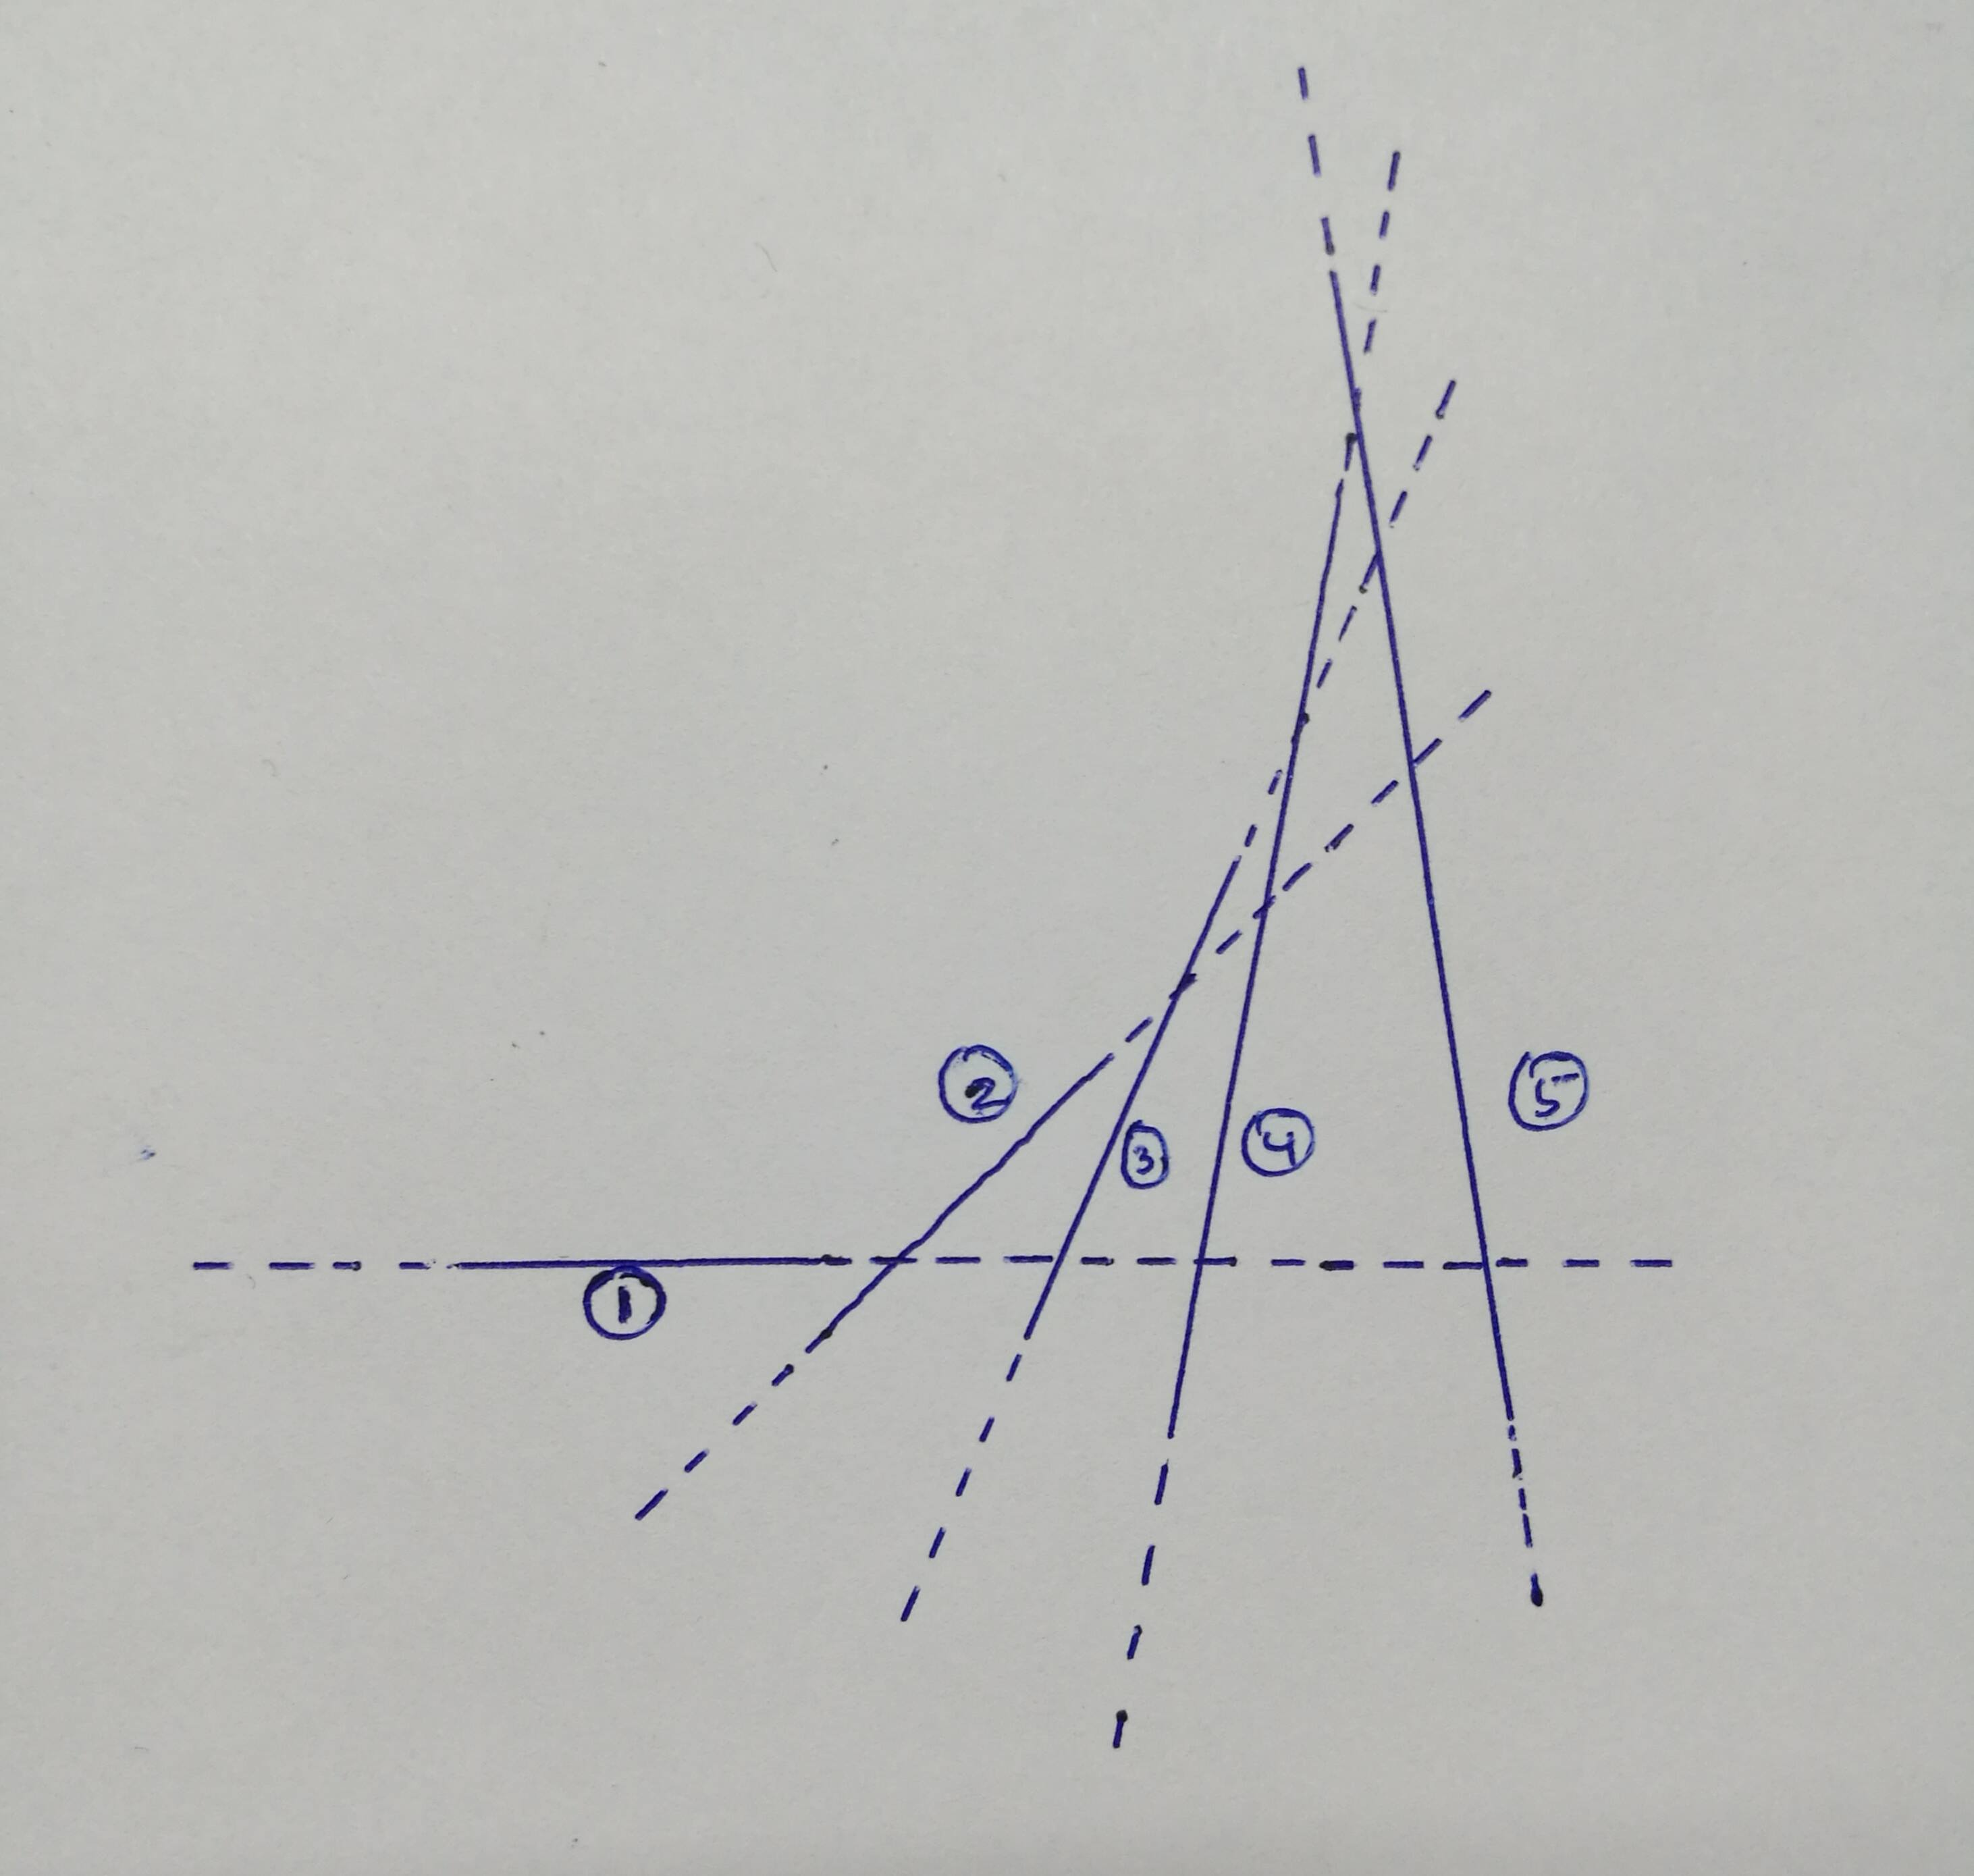
\includegraphics[scale=0.127]{IMG.jpg}
\end{center}
\subsubsection*{2.}
Take any line segment, call it $L$. We will look at all points of intersection which we get after extending this segment towards right, analysis for left side is similar.\\
Label the line segments which intersect the right extended part of $L$ to be $1,2,...,i,...$ in order from left to right. We are considering the intersections after the procedure is completed.\\
\begin{warn}[Observation 1: If line segment $L$ has a point of intersection with line labelled $i$ then $L$ should have been extended before all the line segments labelled $1$ to $i-1$.]\end{warn}
Using Observation 1 and the fact that initially line segments are permuted randomly uniformly(so the probability that any segment is picked first among a subset of size $k$ is $\frac{1}{k}$), the probability that $L$ has a point of intersection with line labelled $i$ is at most $\frac{1}{i}$.\\
Consider random variable $X_i$ taking value $1$ if line segment $i$ intersects with $L$ otherwise $0$.\\
So, $$E[X_i] = P(X_i = 1)*1 + P(X_i = 0)*0 \implies E[X_i] \leq  \frac{1}{i}$$
Let $X$ be the number of points of intersection caused by line segment $L$ when extended towards right.\\
By Linearity of Expectation, 
$$E[X] = \sum_{i=1}^n E[X_i]$$
$$E[X] \leq \sum_{i=1}^n \frac{1}{i}$$
$$E[X] = O(\log n)$$
Similarly, we can get the same bound on the expected number of points of intersection caused by line segment $L$ when extended towards left.\\
Thus expected number of points of intersection caused by the extension of line segment $L$ is $O(\log n)$.\\
\begin{warn}[Observation 2: No two line segments intersected with each other initially, so all points of intersection will be due to extension of line segments.]\end{warn}
Let the total number of points of intersection is $Y$.\\
By Observation 2 and linearity of expectation,
$$E[Y] = n*O(\log n)$$
$$E[Y] = O(n\log n)$$
Thus, for any arbitrary set of $n$ line segments, if we permute them randomly uniformly and then execute the given procedure, the expected number of points of intersection will be $O(n \log n)$.
\pagebreak

% start of Q3
\begin{question}[]
\textbf{Internalizing Backward Analysis and Randomized Incremental Construction (RIC)}
\end{question}
A point $x_i, y_i$ is said to dominate another point $x_j, y_j$ if $x_i > x_j$ and $y_i > y_j$. \\
\textbf{Non dominant point: } A point is said to be non dominant if there is no point in $P$ which dominates it. \\
So we need to find an expected $O(n\log n)$ algorithm to compute all non-dominanted point in $P$. We'll solve this using \textit{Randomized Incremental Construction}, using conflict graphs. \\ \\

Some notations used in analysis are $G_i: $ denotes the conflict graph after $i^{th}$ step, $p_i: $ $i^{th}$ point in our incremental construction, $I_i: $ $i^{th}$ interval on $X$ axis.

\subsubsection*{Conflict Graph Details}
Our conflict graph to solve this problem is based on interval division. Formally at $i^{th}$ stage, conflict graph $C_i$ will store 2-way mapping between set of points and set of intervals (division of $X$ axis). \\ \\ 
If $I_1 = x_0 = x_{min}\rightarrow x_1, I_2 = x_1 \rightarrow x_2, I_k \ldots x_{k-1} \rightarrow x_{k} = x_{max}$ denote the intervals at $i^{th}$ stage ($x_k$ being the point in $P$ having largest $x$ coordinate), then our conflict graph will store which interval, point $p$ belongs to $\forall p \in P$. Also we store a list of all the points belonging to a particular interval. Lastly we'll also store the points which define this interval, ie $x_{i-1}, x_i\in P$ for $I_i, \forall i \in [1,k]$, and the interval height (defined by $H_{i}$ for $I_i$ interval, $H_i =$ maximum value of $y$ coordinate among all points belonging to this interval). For a particular interval, we store the interval which is just left to it, in other words we can get the left neighbor of a interval in $O(1)$. 

Note that these interval heights may change when we proceed incrementally.\\ \\

Some operations and their complexity analysis are:
\begin{itemize}
	\item \textbf{Locating interval of $p_i \in P: $} Well store explicit mapping of interval for each point, so this opearation will take $O(1)$ time.

	\item \textbf{Determining whether $G_{i+1}$ will be different from $G_i: $} Note that $G_{i+1}$ will change only when we change the intervals in our graph. Interval will change if y-coordinate of $p_{i+1}$  is greater than $H_{t}$, where $H_{t}$ is the height of interval at $i^{th}$ stage to which $p_{i+1}$ belong. We can get the interval to which $p_{i+1}$ belongs in $O(1)$, also its height in $O(1)$, we determining whether $G_{i+1}$ will be different will take $O(1)$ time.

	\item \textbf{Updating $G_{i+1}$: } We will update $G_{i+1}$ only if $p_{i+1}$ has height greater than interval height to which $p_{i+1}$ belong to (let this interval be $I_t$). In that case we'll remove all the intervals to the left of $I_t$ having height less than $y_{p_{i+1}}$ (including $I_t$), and introduce 2 new interval $I^1_t, I^2_t$. Lets assume that $I^{'}_1, I^{'}_2, \ldots I^{'}_m$ are the interval to the left of $I_t$ that are removed, then $I^1_t  = (x_{0} \rightarrow x_{p_{i+1}}), I^2_t = (x_{p_{i+1}} \rightarrow x_t)$ (where $x_0$ is the left end of $I^{'}_1$ interval). Height of $I^1_t$ is equal to y-coordinate of $p_{i+1}$ and height of $I^2_t$ is equal to height of $I_t$. We also need to update the mapping of all points belonging to the interval which are affected. Since we store the left neighbor of each interval, this operation can be done efficiently, however it may take $O(n)$ in worst case. 

\end{itemize}
One last thing before we proceed further is that we'll also store the point $p$ which is on the top right corner of a interval. We have seen above that this point $p$ caused creation of this interval. \\
Note that after update we do not keep $i^{th}$ point in the set. So after $i^{th}$ round, in the set we have only $n-i$ points.

\pagebreak

So using these details of implementation as background our algorithm to find non dominant points is:

\begin{algorithm}[H]
\SetAlgoLined
\KwIn{$P = p_1, p_2,\ldots p_n:$ set of n points in $2-D$ plane}
\KwOut{Set of non dominant points in $P$}
  $G_1 = \{ I = \{ I_1 \}, M, S \}$ (initial conflict graph, here $I_1 = (0\rightarrow x_{mx})$, where $x_{mx}$ is maximum $X$ coordinate of all points in $P$) \\
  /* \\
  In subsequent step $M$ will denote the map from set of points to set of intervals \\
  $I$ will denote the set of intervals \\
  $I_k$ will denote $k^{th}$ interval, this will store data for height and interval limit(on $X$ axis).\\
  $H[I_k]$ will denote height of $k^{th}$ interval.\\
  $I_k$ is defined by $x_{k-1} \rightarrow x_k$\\
  $D[I_k]$ will denote the generating point for interval $I_k$ \\
  $S[I_k]$ will denote the set of all points belonging to interval $I_k$ \\
  */ \\
  $S[I_1] = \phi$ \\
  \For{$i \leftarrow 1$ \KwTo $n$} {
  	$M[p_i] \leftarrow I_1$\\
    $S[I_1] \leftarrow S[I_1] \cup {p_i}$ \\
  }
  $I_1 \leftarrow (x_{min}\rightarrow x_{max})$ \\
  $H[I_1] \leftarrow 0$\\
  $D[I_k] \leftarrow p_{x_{mx}}$ // defined by point having maximum value of $X$ coordinate.
 \For{$i \leftarrow 1$ \KwTo $n$} {
 	$I_k$ = $M[p_i]$ \\
 	\uIf{$y_{p_i} > H[I_k]$}{
 			// have to update $G$ \\
      $I_{new} \leftarrow \phi$ \\
      $I_{temp} \leftarrow I_k$ \\
      \While {$H[I_{temp}] \leq y_{p_i}$} {
        $I_{temp} \leftarrow$ left neighbor of $I_{temp}$ \\
        $I_{new} \leftarrow I_{new} \cup {I_{temp}} $ \\
      }
      $I^1_k, I^2_k \leftarrow $ new intervals\\
      update the left, right range and neighbor of $I^1_k, I^2_k$ \\
      $H[I^1_k] \leftarrow y_{p_{i+1}}$ \\
      $H[I^2_k] \leftarrow H[I_k]$ \\
      \For{$I_t  \in I_{new}$} {
        \For {$p \in S[I_t]$} {
          change mapping in $M$ depending on $y$ coordinate. \\
        }
      }
      $D[I^2_k] \leftarrow D[I_k]$ \\
      $D[I^1_k] \leftarrow p_{i+1}$ \\
      Update S value for these 2 interval, but be aware, not to include $i^{th}$ point, because that will give a logarithmic factor compared to linear. \\
 		}
 }
 $T \leftarrow \phi$ \\
 \For{$Q \in I$} {
 	$T = T \cup \{ D[Q] \}$ // include defining point of this interval
 }

 \Return{$T$}
 \caption{RIC based algorithm for finding Non dominant points.}
\end{algorithm}
\pagebreak
\subsubsection*{Time Complexity Analysis}
Running time of $i^{th}$ iteration is of the order of
\begin{itemize}
    \item Number of intervals that are destroyed.
    \item Number of new intervals that are created.
    \item Number of points in the $2$ new interval that get created.
\end{itemize}
Since every intervals destroyed was once created, so the total number of intervals destroyed $<$ total number of intervals created. Hence the total number of intervals created and destroyed = $O(n)$ (since only $2$ intervals get created in each stage). \\ \\
To compute number of points updated in each step we'll use backward analysis. \\
Let $X_i$ be the random variable denoting the number of points for which the map is updated in $i^{th}$ step.
Backward analysis of this problem is exactly same as that of convex hull. \\
$a: $ a subset of $i$ point of $P$ \\
$\epsilon_a: $ first $i$ points of $P$ are some permutation of $a$. \\
\begin{align*}
E[X_i | \epsilon_a] &= n_1 + n_2 \ldots (\dfrac{1}{i}) \\
                    & n_2 + n_3 \ldots (\dfrac{1}{i}) \\
                    & \ldots \\
                    & n_k \ldots (\dfrac{1}{i})\\
\end{align*}
Note that in the last one we have only $n_k$, because for the rightmost interval, we only have created one in the step. \\
Using the above analysis we get $E[X_i | \epsilon_a] \leq \dfrac{2(n-i)}{i}$
Let $S_i$ be the set of all subsets of $P$ of size $i$. \\
$E[X_i] = \sum_{a\in S_i} E[X_i | \epsilon_a]. P(\epsilon_a) \leq \sum_{a\in S_i} \dfrac{2(n-i)}{i}. P(\epsilon_a) = \dfrac{2(n-i)}{i}$ \\ \\
Expected runtime of $i^{th}$ iteration = $E[X_i] + O(1)$ ($O(1)$ is due to creation and deletion of intervals).
\begin{align*}
  &= E[X_i] + O(1) \\
  &= O(\dfrac{n-i}{i})
\end{align*}
Expected running time of the algorithm $\mathbf{= O(n \log n)}$.
\end{document}

